\subsection{Pianificazione dei test}
La consistenza dei test in esecuzioni ripetute è una condizione imperativa, dunque è necessario che essi siano \gl{ripetibili}: un dato test eseguito in un ambiente specifico deve produrre, se fornito un determinato input, sempre gli stessi output. Al fine di garantire ciò, il team 7DOS ha scelto di basarsi sullo standard \gl{ISO/IEC/IEEE 29119}\footnote{ISO/IEC/IEEE 29119 parte 3 sezione 7, IEEE 2013.} per quanto riguarda la pianificazione e documentazione dei test dinamici. Tale standard prevede di definire, per ciascun test o suite di test, una \emph{specifica di test} composta di:
\begin{itemize}
	\item {\textbf{Specifica di progettazione:} definisce le funzionalità del prodotto da testare e le condizioni di test, ovvero l'ambiente di esecuzione e le pre-condizioni (particolari eventi o stati pregressi) necessarie al suo svolgimento;}
	\item {\textbf{Specifica di caso:} definisce l'insieme degli input che si desidera testare, e l'insieme dei risultati attesi per ogni input per una o più funzionalità testate;}
	\item {\textbf{Specifica di procedura:} definisce l'ordine di esecuzione dei test (nel caso di una suite di test), la modalità di svolgimento, ovvero le azioni da compiere e gli input da inserire in modo ordinato, eventuali azioni necessarie per il raggiungimento delle pre-condizioni e la modalità di analisi dei risultati ottenuti.}
\end{itemize}

\newsection{Specifica dei test}
\definecolor{darkgreen}{rgb}{0.0, 0.6, 0.0}
\subsection{Test di accettazione}
\normalsize
\renewcommand{\arraystretch}{1}
\begin{longtable}{|C{2.5cm}|C{2.5cm}|C{2.5cm}|}
	\hline
	\rowcolor{title_row}
	\textbf{\color{title_text}{Test}} & \textbf{\color{title_text}{Requisito}} & \textbf{\color{title_text}{Stato}} \\
	\hline
	\endhead
	{TA-1} & {R0F1} & {NI}\\
	\hline
	{TA-1.1} & {R1F1.1} 
	& {NI}\\
	\hline
	{TA-2} & {R0F2} 
	& {NI}\\
	\hline
	{TA-2.1} & {R0F2.1}
	& {NI}\\
	\hline
	{TA-2.2} & {R0F2.2}
	& {NI}\\
	\hline
	{TA-2.3} & {R1F2.3} 
	& {NI}\\
	\hline
	{TA-3} & {R0F3} 
	& {NI}\\
	\hline
	{TA-3.1} & {R1F3.1}
	& {NI}\\
	\hline
	{TA-4} & {R0F4}
	& {NI}\\
	\hline
	{TA-4.1} & {R1F4.1}
	& {NI}\\
	\hline
	{TA-5} & {R0F5}
	& {NI}\\
	\hline
	{TA-5.1} & {R1F5.1}
	& {NI}\\
	\hline
	{TA-5.2} & {R1F5.2}
	& {NI}\\
	\hline
	{TA-5.3} & {R1F5.3}
	& {NI}\\
	\hline
	{TA-5.4} & {R1F5.4}
	& {NI}\\
	\hline
	{TA-5} & {R1F5.5}
	& {NI}\\
	\hline
	{TA-5.6} & {R1F5.6}
	& {NI}\\
	\hline
	{TA-5.7} & {R1F5.7}
	& {NI}\\
	\hline
	{TA-6} & {R1F6}
	& {NI}\\
	\hline
	{TA-6.1} & {R1F6.1}
	& {NI}\\
	\hline
	{TA-6.2} & {R1F6.2}
	& {NI}\\
	\hline
	{TA-7} & {R1F7}
	& {NI}\\
	\hline
	{TA-7.1} & {R1F7.1}
	& {NI}\\
	\hline
	{TA-7.2} & {R1F7.2}
	& {NI}\\
	\hline
	{TA-7.3} & {R1F7.4}
	& {NI}\\
	\hline
	{TA-7.4} & {R1F7.5}
	& {NI}\\
	\hline
	{TA-7.5} & {R1F7.6}
	& {NI}\\
	\hline
	{TA-7.6} & {R1F7.7}
	& {NI}\\
	\hline
	{TA-8} & {R2F8}
	& {NI}\\
	\hline
	{TA-9} & {R2F9}
	& {NI}\\
	\hline
	{TA-10} & {R2F10}
	& {NI}\\
	\hline
	{TA-10.1} & {R2F10.1}
	& {NI}\\
	\hline
	{TA-10.2} & {R2F10.2}
	& {NI}\\
	\hline
	{TA-10.4} & {R2F10.4}
	& {NI}\\
	\hline
	{TA-10.5} & {R2F10.5}
	& {NI}\\
	\hline
	{TA-10.6} & {R2F10.6}
	& {NI}\\
	\hline
	\caption{Riassunto test di accettazione}
	\label{tabella:riassunto ta}
\end{longtable}
\normalsize
\renewcommand{\arraystretch}{1}
\begin{figure} [H]
	\centering
	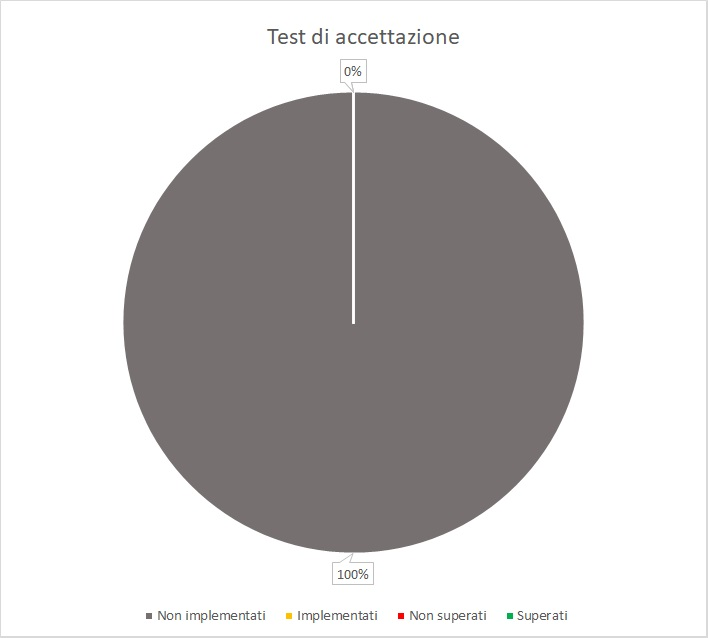
\includegraphics[scale=1]{Img/TA}
	\caption{Resoconto test di accettazione}\label{}
\end{figure}
\newpage

\subsection{Test di sistema}
\begin{longtable}{|C{2.5cm}|C{2.5cm}|C{2.5cm}|}
	\hline
	\rowcolor{title_row}
	\textbf{\color{title_text}{Test}} & \textbf{\color{title_text}{Requisito}} & \textbf{\color{title_text}{Stato}} \\
	\hline
	\endhead
	{TS-1} & {R0F1} & \textcolor{darkgreen}{\textbf{S}}\\
	\hline
	{TS-1.1} & {R1F1.1}& {NI}\\
	\hline
	{TS-2} & {R0F2}  & {NI}\\
	\hline
	{TS-2.1} & {R0F2.1}  & {NI}\\
	\hline
	{TS-2.2} & {R0F2.2} & {NI}\\
	\hline
	{TS-2.3} & {R1F2.3}  & \textcolor{darkgreen}{\textbf{S}}\\
	\hline
	{TS-3} & {R0F3} & {NI}\\
	\hline
	{TS-3.1} & {R1F3.1} & {NI}\\
	\hline
	{TS-4} & {R0F4} & {NI}\\
	\hline
	{TS-4.1} & {R1F4.1} & \textcolor{darkgreen}{\textbf{S}}\\
	\hline
	{TS-5} & {R0F5} & {NI}\\
	\hline
	{TS-5.1} & {R1F5.1} & \textcolor{darkgreen}{\textbf{S}}\\
	\hline
	{TS-5.2} & {R1F5.2}  & \textcolor{darkgreen}{\textbf{S}}\\
	\hline
	{TS-5.3} & {R1F5.3} & \textcolor{darkgreen}{\textbf{S}}\\
	\hline
	{TS-5.4} & {R1F5.4} & \textcolor{darkgreen}{\textbf{S}}\\
	\hline
	{TS-5.5} & {R1F5.5} & \textcolor{darkgreen}{\textbf{S}}\\
	\hline
	{TS-5.6} & {R1F5.6} & \textcolor{darkgreen}{\textbf{S}}\\
	\hline
	{TS-5.6.1} & {R0F5.6.1} & {NI}\\
	\hline
	{TS-5.6.2} & {R1F5.6.2} & {NI}\\
	\hline
	{TS-5.6.3} & {R1F5.6.3} & \textcolor{darkgreen}{\textbf{S}}\\
	\hline
	{TS-5.7} & {R1F5.7} & \textcolor{darkgreen}{\textbf{S}}\\
	\hline
	{TS-5.7.1} & {R1F5.7.1} & \textcolor{darkgreen}{\textbf{S}}\\
	\hline
	{TS-6} & {R1F6} & \textcolor{darkgreen}{\textbf{S}}\\
	\hline
	{TS-6.1} & {R1F6.1} & \textcolor{darkgreen}{\textbf{S}}\\
	\hline
	{TS-6.1.1} & {R1F6.1.1} & \textcolor{darkgreen}{\textbf{S}}\\
	\hline
	{TS-6.1.2} & {R1F6.1.2} & \textcolor{darkgreen}{\textbf{S}}\\
	\hline
	{TS-6.1.3} & {R1F6.1.3}  & \textcolor{darkgreen}{\textbf{S}}\\
	\hline
	{TS-6.2} & {R1F6.2} & \textcolor{darkgreen}{\textbf{S}}\\
	\hline
	{TS-7} & {R1F7} & {NI}\\
	\hline
	{TS-7.1} & {R1F7.1} & {NI}\\
	\hline
	{TS-7.11} & {R1F7.1.1} & {NI}\\
	\hline
	{TS-7.1.2} & {R1F7.1.2} & {NI}\\
	\hline
	{TS-7.1.3} & {R1F7.1.3} & {NI}\\
	\hline
	{TS-7.1.4} & {R1F7.1.4} & {NI}\\
	\hline
	{TS-7.1.4.1} & {R1F7.1.4.1} & {NI}\\
	\hline
	{TS-7.1.4.2} & {R1F7.1.4.2} & {NI}\\
	\hline
	{TS-7.1.4.3} & {R1F7.1.4.3} & {NI}\\
	\hline
	{TS-7.2} & {R1F7.2} & {NI}\\
	\hline
	{TS-7.2.1} & {R1F7.2.1} & {NI}\\
	\hline
	{TS-7.2.2} & {R1F7.2.2} & {NI}\\
	\hline
	{TS-7.2.2.1} & {R1F7.2.2.1} & {NI}\\
	\hline
	{TS-7.2.2.2} & {R1F7.2.2.2} & {NI}\\
	\hline
	{TS-7.2.2.3} & {R1F7.2.2.3} & {NI}\\
	\hline
	{TS-7.2.2.4} & {R1F7.2.2.4} & {NI}\\
	\hline
	{TS-7.3} & {R1F7.3} & {NI}\\
	\hline
	{TS-7.4} & {R1F7.4} & {NI}\\
	\hline
	{TS-7.4.1} & {R1F7.4.1} & {NI}\\
	\hline
	{TS-7.4.2} & {R1F7.4.2} & {NI}\\
	\hline
	{TS-7.5} & {R1F7.5} & {NI}\\
	\hline
	{TS-7.6} & {R1F7.6} & {NI}\\
	\hline
	{TS-7.6.1} & {R1F7.6.1} & {NI}\\
	\hline
	{TS-7.6.2} & {R1F7.6.2} & {NI}\\
	\hline
	{TS-7.7} & {R1F7.7} & {NI}\\
	\hline
	{TS-7.7.1} & {R1F7.7.1} & {NI}\\
	\hline
	{TS-7.7.2} & {R1F7.7.2} & {NI}\\
	\hline
	{TS-7.7.3} & {R1F7.7.3} & {NI}\\
	\hline
	{TS-7.7.4} & {R1F7.7.4} & {NI}\\
	\hline
	{TS-8} & {R2F8} & {NI}\\
	\hline
	{TS-9} & {R2F9} & {NI}\\
	\hline
	{TS-10} & {R2F10} & \textcolor{darkgreen}{\textbf{S}}\\
	\hline
	{TS-10.1} & {R2F10.1} & \textcolor{darkgreen}{\textbf{S}}\\
	\hline
	{TS-10.2} & {R2F10.2} & \textcolor{darkgreen}{\textbf{S}}\\
	\hline
	{TS-10.3} & {R2F10.3} & \textcolor{darkgreen}{\textbf{S}}\\
	\hline
	{TS-10.3.1} & {R2F10.3.1} & \textcolor{darkgreen}{\textbf{S}}\\
	\hline
	{TS-10.3.2} & {R2F10.3.2} & \textcolor{darkgreen}{\textbf{S}}\\
	\hline
	{TS-10.3.3} & {R2F10.3.3} & \textcolor{darkgreen}{\textbf{S}}\\
	\hline
	{TS-10.3.4} & {R2F10.3.4} & \textcolor{darkgreen}{\textbf{S}}\\
	\hline
	{TS-10.3.5} & {R2F10.3.5} & \textcolor{darkgreen}{\textbf{S}}\\
	\hline
	{TS-10.4} & {R2F10.4} & \textcolor{darkgreen}{\textbf{S}}\\
	\hline
	{TS-10.4.1} & {R2F10.4.1} & \textcolor{darkgreen}{\textbf{S}}\\
	\hline
	{TS-10.4.2} & {R2F10.4.2} & \textcolor{darkgreen}{\textbf{S}}\\
	\hline
	{TS-10.4.3} & {R2F10.4.3} & \textcolor{darkgreen}{\textbf{S}}\\
	\hline
	{TS-10.4.3.1} & {R2F10.4.3.1} & \textcolor{darkgreen}{\textbf{S}}\\
	\hline
	{TS-10.4.3.2} & {R2F10.4.3.2} & \textcolor{darkgreen}{\textbf{S}}\\
	\hline
	{TS-10.4.3.3} & {R2F10.4.3.3} & \textcolor{darkgreen}{\textbf{S}}\\
	\hline
	{TS-10.5} & {R2F10.5} & \textcolor{darkgreen}{\textbf{S}}\\
	\hline
	{TS-10.6} & {R2F10.6} & \textcolor{darkgreen}{\textbf{S}}\\
	\hline
	\caption{Riassunto test di sistema}
	\label{tabella:riassunto TS}
\end{longtable}
\renewcommand{\arraystretch}{1}
\begin{figure} [H]
	\centering
	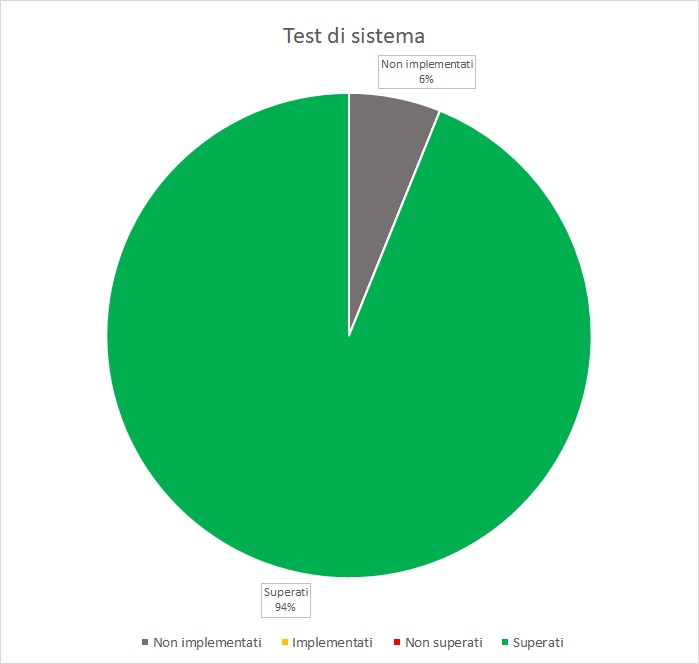
\includegraphics[scale=1]{Img/TS}
	\caption{Resoconto test di sistema}\label{}
\end{figure}
\newpage

\subsection{Test di integrazione}
\normalsize
\renewcommand{\arraystretch}{1}
\begin{longtable}{|C{2.5cm}|C{4.5cm}|C{2.5cm}|}
	\hline
	\rowcolor{title_row}
	\textbf{\color{title_text}{Test}} & \textbf{\color{title_text}{Componente}} & \textbf{\color{title_text}{Stato}} \\
	\hline
	\endhead
	{TI-1} & Client - Grafana. & \textcolor{darkgreen}{\textbf{S}}\\
	\hline
	{TI-2} & Grafana - \gl{InfluxDB} & \textcolor{darkgreen}{\textbf{S}}\\
	\hline
	{TI-3} & Grafana - JsBayes & \textcolor{darkgreen}{\textbf{S}}\\
	\hline
	{TI-4} & Grafana - Raintank & \textcolor{darkgreen}{\textbf{S}}\\
	\hline
	\caption{Riassunto test di integrazione}
	\label{tabella:riassunto ta}
\end{longtable}
\renewcommand{\arraystretch}{1}
\begin{figure} [H]
	\centering
	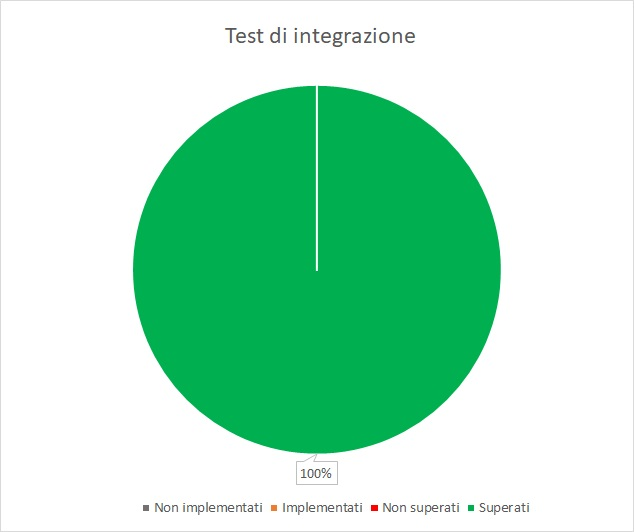
\includegraphics[scale=1]{Img/TI}
	\caption{Resoconto test di integrazione}\label{}
\end{figure}
\newpage

\subsection{Test di unità}
\begin{longtable}{|C{2.5cm}|C{2.5cm}|}
	\hline
	\rowcolor{title_row}
	\textbf{\color{title_text}{Test}} & \textbf{\color{title_text}{Stato}} \\
	\hline
	\endhead
	{TU-1} & \textcolor{darkgreen}{\textbf{S}}\\
	\hline
	{TU-2} & \textcolor{darkgreen}{\textbf{S}}\\
	\hline
	{TU-3} & \textcolor{darkgreen}{\textbf{S}}\\
	\hline
	{TU-4} & \textcolor{darkgreen}{\textbf{S}}\\
	\hline
	{TU-5} & \textcolor{darkgreen}{\textbf{S}}\\
	\hline
	{TU-6} & \textcolor{darkgreen}{\textbf{S}}\\
	\hline
	{TU-7} & \textcolor{darkgreen}{\textbf{S}}\\
	\hline
	{TU-8} & \textcolor{darkgreen}{\textbf{S}}\\
	\hline
	{TU-9} & \textcolor{darkgreen}{\textbf{S}}\\
	\hline
	{TU-10} & \textcolor{darkgreen}{\textbf{S}}\\
	\hline
	{TU-11} & \textcolor{darkgreen}{\textbf{S}}\\
	\hline
	{TU-12} & \textcolor{darkgreen}{\textbf{S}}\\
	\hline
	{TU-13} & \textcolor{darkgreen}{\textbf{S}}\\
	\hline
	{TU-14} & \textcolor{darkgreen}{\textbf{S}}\\
	\hline
	{TU-15} & \textcolor{darkgreen}{\textbf{S}}\\
	\hline
	{TU-16} & \textcolor{darkgreen}{\textbf{S}}\\
	\hline
	{TU-17} & \textcolor{darkgreen}{\textbf{S}}\\
	\hline
	{TU-18} & \textcolor{darkgreen}{\textbf{S}}\\
	\hline
	{TU-19} & \textcolor{darkgreen}{\textbf{S}}\\
	\hline
	{TU-20} & \textcolor{darkgreen}{\textbf{S}}\\
	\hline
	{TU-21} & \textcolor{darkgreen}{\textbf{S}}\\
	\hline
	{TU-22} & \textcolor{darkgreen}{\textbf{S}}\\
	\hline
	{TU-23} & \textcolor{darkgreen}{\textbf{S}}\\
	\hline
	{TU-24} & \textcolor{darkgreen}{\textbf{S}}\\
	\hline
	{TU-25} & \textcolor{darkgreen}{\textbf{S}}\\
	\hline
	{TU-26} & \textcolor{darkgreen}{\textbf{S}}\\
	\hline
	{TU-27} & \textcolor{darkgreen}{\textbf{S}}\\
	\hline
	{TU-28} & \textcolor{darkgreen}{\textbf{S}}\\
	\hline
	{TU-29} & \textcolor{darkgreen}{\textbf{S}}\\
	\hline
	{TU-30} & \textcolor{darkgreen}{\textbf{S}}\\
	\hline
	{TU-31} & \textcolor{darkgreen}{\textbf{S}}\\
	\hline
	{TU-32} & \textcolor{darkgreen}{\textbf{S}}\\
	\hline
	{TU-33} & \textcolor{darkgreen}{\textbf{S}}\\
	\hline
	{TU-34} & \textcolor{darkgreen}{\textbf{S}}\\
	\hline
	{TU-35} & \textcolor{darkgreen}{\textbf{S}}\\
	\hline
	{TU-36} & \textcolor{darkgreen}{\textbf{S}}\\
	\hline
	{TU-37} & \textcolor{darkgreen}{\textbf{S}}\\
	\hline
	{TU-38} & \textcolor{darkgreen}{\textbf{S}}\\
	\hline
	{TU-39} & \textcolor{darkgreen}{\textbf{S}}\\
	\hline
	{TU-40} & \textcolor{darkgreen}{\textbf{S}}\\
	\hline
	{TU-41} & \textcolor{darkgreen}{\textbf{S}}\\
	\hline
	{TU-42} & \textcolor{darkgreen}{\textbf{S}}\\
	\hline
	{TU-43} & \textcolor{darkgreen}{\textbf{S}}\\
	\hline
	{TU-44} & \textcolor{darkgreen}{\textbf{S}}\\
	\hline
	{TU-45} & \textcolor{darkgreen}{\textbf{S}}\\
	\hline
	{TU-46} & \textcolor{darkgreen}{\textbf{S}}\\
	\hline
	{TU-47} & \textcolor{darkgreen}{\textbf{S}}\\
	\hline
	{TU-48} & \textcolor{darkgreen}{\textbf{S}}\\
	\hline
	{TU-49} & \textcolor{darkgreen}{\textbf{S}}\\
	\hline
	{TU-50} & \textcolor{darkgreen}{\textbf{S}}\\
	\hline
	{TU-51} & \textcolor{darkgreen}{\textbf{S}}\\
	\hline
	{TU-52} & \textcolor{darkgreen}{\textbf{S}}\\
	\hline
	{TU-53} & \textcolor{darkgreen}{\textbf{S}}\\
	\hline
	{TU-54} & \textcolor{darkgreen}{\textbf{S}}\\
	\hline
	\caption{Riassunto test di unità}
	\label{tabella:riassunto tu}
\end{longtable}
\renewcommand{\arraystretch}{1}
\begin{figure} [H]
	\centering
	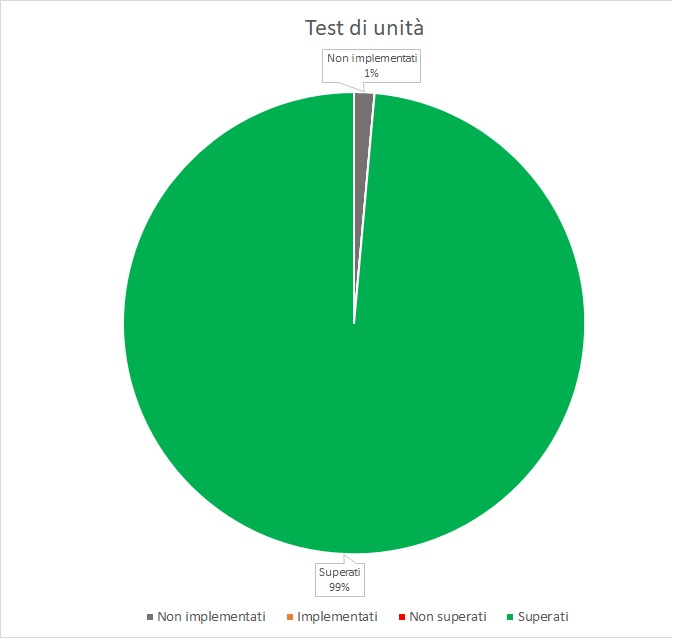
\includegraphics[scale=0.7]{Img/TU}
	\caption{Resoconto test di unità}\label{}
\end{figure}


\pagebreak